% Options for packages loaded elsewhere
\PassOptionsToPackage{unicode}{hyperref}
\PassOptionsToPackage{hyphens}{url}
%
\documentclass[
  oneside,
  open=any]{scrbook}

\usepackage{amsmath,amssymb}
\usepackage{iftex}
\ifPDFTeX
  \usepackage[T1]{fontenc}
  \usepackage[utf8]{inputenc}
  \usepackage{textcomp} % provide euro and other symbols
\else % if luatex or xetex
  \usepackage{unicode-math}
  \defaultfontfeatures{Scale=MatchLowercase}
  \defaultfontfeatures[\rmfamily]{Ligatures=TeX,Scale=1}
\fi
\usepackage{lmodern}
\ifPDFTeX\else  
    % xetex/luatex font selection
\fi
% Use upquote if available, for straight quotes in verbatim environments
\IfFileExists{upquote.sty}{\usepackage{upquote}}{}
\IfFileExists{microtype.sty}{% use microtype if available
  \usepackage[]{microtype}
  \UseMicrotypeSet[protrusion]{basicmath} % disable protrusion for tt fonts
}{}
\makeatletter
\@ifundefined{KOMAClassName}{% if non-KOMA class
  \IfFileExists{parskip.sty}{%
    \usepackage{parskip}
  }{% else
    \setlength{\parindent}{0pt}
    \setlength{\parskip}{6pt plus 2pt minus 1pt}}
}{% if KOMA class
  \KOMAoptions{parskip=half}}
\makeatother
\usepackage{xcolor}
\setlength{\emergencystretch}{3em} % prevent overfull lines
\setcounter{secnumdepth}{5}
% Make \paragraph and \subparagraph free-standing
\makeatletter
\ifx\paragraph\undefined\else
  \let\oldparagraph\paragraph
  \renewcommand{\paragraph}{
    \@ifstar
      \xxxParagraphStar
      \xxxParagraphNoStar
  }
  \newcommand{\xxxParagraphStar}[1]{\oldparagraph*{#1}\mbox{}}
  \newcommand{\xxxParagraphNoStar}[1]{\oldparagraph{#1}\mbox{}}
\fi
\ifx\subparagraph\undefined\else
  \let\oldsubparagraph\subparagraph
  \renewcommand{\subparagraph}{
    \@ifstar
      \xxxSubParagraphStar
      \xxxSubParagraphNoStar
  }
  \newcommand{\xxxSubParagraphStar}[1]{\oldsubparagraph*{#1}\mbox{}}
  \newcommand{\xxxSubParagraphNoStar}[1]{\oldsubparagraph{#1}\mbox{}}
\fi
\makeatother

\providecommand{\tightlist}{%
  \setlength{\itemsep}{0pt}\setlength{\parskip}{0pt}}\usepackage{longtable,booktabs,array}
\usepackage{calc} % for calculating minipage widths
% Correct order of tables after \paragraph or \subparagraph
\usepackage{etoolbox}
\makeatletter
\patchcmd\longtable{\par}{\if@noskipsec\mbox{}\fi\par}{}{}
\makeatother
% Allow footnotes in longtable head/foot
\IfFileExists{footnotehyper.sty}{\usepackage{footnotehyper}}{\usepackage{footnote}}
\makesavenoteenv{longtable}
\usepackage{graphicx}
\makeatletter
\def\maxwidth{\ifdim\Gin@nat@width>\linewidth\linewidth\else\Gin@nat@width\fi}
\def\maxheight{\ifdim\Gin@nat@height>\textheight\textheight\else\Gin@nat@height\fi}
\makeatother
% Scale images if necessary, so that they will not overflow the page
% margins by default, and it is still possible to overwrite the defaults
% using explicit options in \includegraphics[width, height, ...]{}
\setkeys{Gin}{width=\maxwidth,height=\maxheight,keepaspectratio}
% Set default figure placement to htbp
\makeatletter
\def\fps@figure{htbp}
\makeatother

% delete. this is for the example w CZ diacritics
\usepackage{babel}
\babelprovide[import]{czech}
\makeatletter
\@ifpackageloaded{caption}{}{\usepackage{caption}}
\AtBeginDocument{%
\ifdefined\contentsname
  \renewcommand*\contentsname{Table of contents}
\else
  \newcommand\contentsname{Table of contents}
\fi
\ifdefined\listfigurename
  \renewcommand*\listfigurename{List of Figures}
\else
  \newcommand\listfigurename{List of Figures}
\fi
\ifdefined\listtablename
  \renewcommand*\listtablename{List of Tables}
\else
  \newcommand\listtablename{List of Tables}
\fi
\ifdefined\figurename
  \renewcommand*\figurename{Figure}
\else
  \newcommand\figurename{Figure}
\fi
\ifdefined\tablename
  \renewcommand*\tablename{Table}
\else
  \newcommand\tablename{Table}
\fi
}
\@ifpackageloaded{float}{}{\usepackage{float}}
\floatstyle{ruled}
\@ifundefined{c@chapter}{\newfloat{codelisting}{h}{lop}}{\newfloat{codelisting}{h}{lop}[chapter]}
\floatname{codelisting}{Listing}
\newcommand*\listoflistings{\listof{codelisting}{List of Listings}}
\makeatother
\makeatletter
\makeatother
\makeatletter
\@ifpackageloaded{caption}{}{\usepackage{caption}}
\@ifpackageloaded{subcaption}{}{\usepackage{subcaption}}
\makeatother

\usepackage{hyphenat}
\usepackage{ifthen}
\usepackage{calc}
\usepackage{calculator}

\usepackage{graphicx}
\usepackage{wallpaper}

\usepackage{geometry}

\usepackage{graphicx}
\usepackage{geometry}
\usepackage{afterpage}
\usepackage{tikz}
\usetikzlibrary{calc}
\usetikzlibrary{fadings}
\usepackage[pagecolor=none]{pagecolor}


% Set the titlepage font families







% Set the coverpage font families
\usepackage{fontspec}
\newfontfamily{\coverpagetitlefont}{QTDublinIrish.otf}
\usepackage{fontspec}
\newfontfamily{\coverpagefooterfont}{QTDublinIrish.otf}


\ifLuaTeX
  \usepackage{selnolig}  % disable illegal ligatures
\fi
\usepackage{bookmark}

\IfFileExists{xurl.sty}{\usepackage{xurl}}{} % add URL line breaks if available
\urlstyle{same} % disable monospaced font for URLs
\hypersetup{
  pdftitle={Inchainge Game Assistance - Study},
  pdfauthor={Christiaan Verhoef; Michiel Steeman},
  hidelinks,
  pdfcreator={LaTeX via pandoc}}


\title{Inchainge Game Assistance - Study}
\usepackage{etoolbox}
\makeatletter
\providecommand{\subtitle}[1]{% add subtitle to \maketitle
  \apptocmd{\@title}{\par {\large #1 \par}}{}{}
}
\makeatother
\subtitle{Integrating Sustainability Reporting with Agent-Based Tools}
\author{Christiaan Verhoef \and Michiel Steeman}
\date{}

\begin{document}
%%%%% begin titlepage extension code

  \begin{frontmatter}

\begin{titlepage}
% This is a combination of Pandoc templating and LaTeX
% Pandoc templating https://pandoc.org/MANUAL.html#templates
% See the README for help

\thispagestyle{empty}

\newgeometry{top=-100in}

% Page color
\definecolor{pgcolor}{HTML}{F6D5A8}
\pagecolor{pgcolor}\afterpage{\nopagecolor}

\newcommand{\coverauthorstyle}[1]{{#1}}

\begin{tikzpicture}[remember picture, overlay, inner sep=0pt, outer sep=0pt]

\tikzfading[name=fadeout, inner color=transparent!0,outer color=transparent!100]
\tikzfading[name=fadein, inner color=transparent!100,outer color=transparent!0]
\node[ scope fading=north, anchor=south west, rotate=0.0, opacity=1.0] at ($(current page.south west)+(0.0, 0.0)$) {
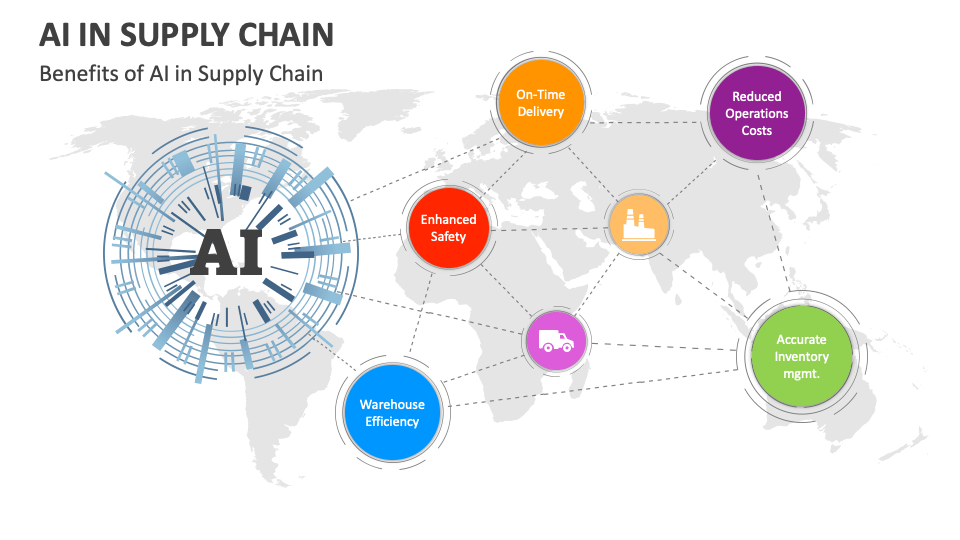
\includegraphics[width=\paperwidth, keepaspectratio]{img/TheGreatWaveoffKanagawa.png}};

% Title
\newcommand{\titlelocationleft}{0.8\paperwidth}
\newcommand{\titlelocationbottom}{10in}
\newcommand{\titlealign}{right}

\begin{scope}{%
\fontsize{40}{48.0}\selectfont
\coverpagetitlefont
\node[anchor=north
east, align=right, rotate=0] (Title1) at ($(current page.south west)+(\titlelocationleft,\titlelocationbottom)$)  [text width = 0.7\paperwidth]  {{\nohyphens{quarto\_titlepages}}};
}
\end{scope}

% Footer
\newcommand{\footerlocationleft}{0.8\paperwidth}
\newcommand{\footerlocationbottom}{9.5in}
\newcommand{\footerlocationalign}{right}

\begin{scope}
{%
\fontsize{20}{24.0}\selectfont
 \coverpagefooterfont
\node[anchor=north east, align=right, rotate=0] (Footer1) at %
($(current page.south west)+(\footerlocationleft,\footerlocationbottom)$)  [text width = 0.7\paperwidth]  {{\nohyphens{Templates
for title pages and covers}}};
}
\end{scope}

\end{tikzpicture}
\clearpage
\restoregeometry
\input{tex/copyright.tex}
\clearpage

%%% TITLE PAGE START

% Set up alignment commands
%Page
\newcommand{\titlepagepagealign}{
\ifthenelse{\equal{left}{right}}{\raggedleft}{}
\ifthenelse{\equal{left}{center}}{\centering}{}
\ifthenelse{\equal{left}{left}}{\raggedright}{}
}


\newcommand{\titleandsubtitle}{
% Title and subtitle
{{\large{\bfseries{\nohyphens{Inchainge Game Assistance - Study}}}}\par
}%

\vspace{\betweentitlesubtitle}
{
{\large{\textit{\nohyphens{Integrating Sustainability Reporting with
Agent-Based Tools}}}}\par
}}
\newcommand{\titlepagetitleblock}{
\titleandsubtitle
}

\newcommand{\authorstyle}[1]{{\large{#1}}}

\newcommand{\affiliationstyle}[1]{{\large{#1}}}

\newcommand{\titlepageauthorblock}{
{\authorstyle{\nohyphens{Christiaan
Verhoef}{\textsuperscript{1}}\textsuperscript{,}{\textsuperscript{2}}\textsuperscript{,}{\textsuperscript{3}}\textsuperscript{,}{\textsuperscript{4}}\textsuperscript{,}{\textsuperscript{*}} and \nohyphens{Michiel
Steeman}{\textsuperscript{5}}\textsuperscript{,}{\textsuperscript{6}}\textsuperscript{,}{\textsuperscript{*}}}}}

\newcommand{\titlepageaffiliationblock}{
\hangindent=1em
\hangafter=1
{\affiliationstyle{
{1}.~Social Chicken,~Thorbeckelaan 35F
\par\hangindent=1em\hangafter=1{2}.~Value Chain Hackers,~Innovation Lab,
Netherlands
\par\hangindent=1em\hangafter=1{3}.~Windesheim University of Applied
Sciences,~Campus 2-6, Zwolle, Netherlands
\par\hangindent=1em\hangafter=1{4}.~University of Minnesota,~Department
of Mathematics
\par\hangindent=1em\hangafter=1{5}.~Inchainge B.V.,~Emmalaan 5, 3732 GM
De Bilt, Netherlands
\par\hangindent=1em\hangafter=1{6}.~Weindesheim University of Applied
Sciences,~Campus 2-6, Zwolle, Netherlands


\vspace{1\baselineskip} 
* \textit{Correspondence:}~Christiaan Verhoef~cg.verhoef@windesheim.nl
* \textit{Correspondence:}~Michiel Steeman~ma.steeman@windesheim.nl
}}
}
\newcommand{\headerstyled}{%
{Value Chain Hackers}
}
\newcommand{\footerstyled}{%
{\large{Open Source Supply Chain Tools\\
\url{https://github.com/valuechainhackers}\strut \\}}
}
\newcommand{\datestyled}{%
{}
}


\newcommand{\titlepageheaderblock}{\headerstyled}

\newcommand{\titlepagefooterblock}{
\footerstyled
}

\newcommand{\titlepagedateblock}{
\datestyled
}

%set up blocks so user can specify order
\newcommand{\titleblock}{\newlength{\betweentitlesubtitle}
\setlength{\betweentitlesubtitle}{\baselineskip}
{

{\titlepagetitleblock}
}

\vspace{4\baselineskip}
}

\newcommand{\authorblock}{{\titlepageauthorblock}

\vspace{2\baselineskip}
}

\newcommand{\affiliationblock}{{\titlepageaffiliationblock}

\vspace{1pt}
}

\newcommand{\logoblock}{{
\includegraphics[width=0.25\textheight]{img/logo.png}}

\vspace{2\baselineskip}
}

\newcommand{\footerblock}{{\titlepagefooterblock}

\vspace{1pt}
}

\newcommand{\dateblock}{}

\newcommand{\headerblock}{{\titlepageheaderblock

\vspace{0pt}
}}
\newgeometry{top=3in,bottom=1in,right=1in,left=1in}
% background image
\newlength{\bgimagesize}
\setlength{\bgimagesize}{0.5\paperwidth}
\LENGTHDIVIDE{\bgimagesize}{\paperwidth}{\theRatio} % from calculator pkg
\ThisULCornerWallPaper{\theRatio}{img/corner-bg.png}

\thispagestyle{empty} % no page numbers on titlepages


\newcommand{\vrulecode}{\rule{\vrulewidth}{\textheight}}
\newlength{\vrulewidth}
\setlength{\vrulewidth}{1pt}
\newlength{\B}
\setlength{\B}{\ifdim\vrulewidth > 0pt 0.05\textwidth\else 0pt\fi}
\newlength{\minipagewidth}
\ifthenelse{\equal{left}{left} \OR \equal{left}{right} }
{% True case
\setlength{\minipagewidth}{\textwidth - \vrulewidth - \B - 0.1\textwidth}
}{
\setlength{\minipagewidth}{\textwidth - 2\vrulewidth - 2\B - 0.1\textwidth}
}
\ifthenelse{\equal{left}{left} \OR \equal{left}{leftright}}
{% True case
\raggedleft % needed for the minipage to work
\vrulecode
\hspace{\B}
}{%
\raggedright % else it is right only and width is not 0
}
% [position of box][box height][inner position]{width}
% [s] means stretch out vertically; assuming there is a vfill
\begin{minipage}[b][\textheight][s]{\minipagewidth}
\titlepagepagealign
\titleblock

\authorblock

\affiliationblock

\vfill

\logoblock

\footerblock
\par

\end{minipage}\ifthenelse{\equal{left}{right} \OR \equal{left}{leftright} }{
\hspace{\B}
\vrulecode}{}
\clearpage
\restoregeometry
%%% TITLE PAGE END

\begin{center}
    \thispagestyle{empty}
    \vspace*{\fill}
    \Huge{\textit{This project is dedicated to those who believed in the power of collaboration and innovation, especially Michiel Steeman, whose unwavering support has been the spark that ignited its creation.}}
    \vspace*{\fill}
\end{center}
\clearpage
\end{titlepage}
\setcounter{page}{1}
\end{frontmatter}

%%%%% end titlepage extension code

\renewcommand*\contentsname{Table of contents}
{
\setcounter{tocdepth}{2}
\tableofcontents
}
\listoffigures
\listoftables

\mainmatter
\chapter{Introduction}\label{introduction}

Supply chain finance plays a pivotal role in aligning sustainable
business practices with economic profitability. In this document, we
explore how digital workspaces and AI tools can revolutionize
transparency and sustainability reporting in supply chains. By
integrating agent-based systems with forensic methodologies, businesses
can optimize operations, reduce waste, and ensure long-term viability.

Lorem ipsum dolor sit amet, consectetur adipiscing elit. Proin eu tempor
velit. Fusce accumsan ultrices fringilla. Praesent sed odio mi. Mauris
non ligula turpis. Duis posuere lacus nec diam interdum dictum suscipit
magna molestie. Vestibulum nibh dolor, interdum eget rhoncus ut, sodales
eget justo.

\chapter{Supporting Theory}\label{supporting-theory}

The central limit theorem in agent-based simulations can be applied as
follows. Let \(X_1, X_2, \ldots, X_n\) represent independent decisions
made by agents in a supply chain network:

\begin{equation}\phantomsection\label{eq-clt}{
S_n = \frac{X_1 + X_2 + \cdots + X_n}{n}
      = \frac{1}{n}\sum_{i=1}^{n} X_i
}\end{equation}

As the number of agents increases, the overall performance converges
toward a steady state, which approximates optimal resource allocation
within the supply chain, as demonstrated in Equation~\ref{eq-clt}.

\chapter{Materials and Methods}\label{materials-and-methods}

Our primary toolset consists of agent-based modeling, forensic EDRM
methodologies, and real-time reporting systems integrated into a shared
workspace. We utilized the OpenWebGUI platform and Agent Chef for
training and managing AI-driven supply chain models. Participants in
this study used real-time dashboards to track key performance
indicators, enabling swift adjustments based on real-world data.

\chapter{Study Area}\label{study-area}

The study took place within a simulated environment modeled after
real-world supply chains. Workspaces were mapped out using co-creation
digital platforms, allowing for collaborative interactions between
various industry professionals and AI agents.

\begin{figure}

\centering{


\includegraphics{img/vch-logo.png}

}

\caption{\label{fig-logo}The collaborative workspace}

\end{figure}%

Figure~\ref{fig-logo} shows the virtual layout used by participants to
visualize data streams in the supply chain network.

\chapter{Results}\label{results}

\begin{longtable}[]{@{}lr@{}}
\caption{Table of Key Performance
Indicators.}\label{tbl-results}\tabularnewline
\toprule\noalign{}
Parameter & Value \\
\midrule\noalign{}
\endfirsthead
\toprule\noalign{}
Parameter & Value \\
\midrule\noalign{}
\endhead
\bottomrule\noalign{}
\endlastfoot
Financial ROI & 24\% \\
Waste Reduced & 15\% \\
Time Saved & 10\% \\
\end{longtable}

\chapter{Discussion}\label{discussion}

Our findings suggest that integrating agent-based tools into supply
chain finance operations can dramatically improve efficiency, reduce
resource waste, and enhance sustainability reporting. The Value Chain
Hackers project demonstrated the potential for real-time data to drive
decision-making and foster a culture of transparency.

Curabitur efficitur in risus quis egestas. Suspendisse potenti. In
ultricies ante accumsan lectus rhoncus, vel pharetra sem convallis.

\chapter{Conclusion}\label{conclusion}

The alignment of AI tools with sustainability and finance goals presents
a unique opportunity for businesses to both enhance their market
viability and meet environmental standards. Further research into
AI-driven supply chain reporting systems is crucial for ensuring
continued progress toward sustainability goals.

\chapter{Author Contributions}\label{author-contributions}

\begin{itemize}
\tightlist
\item
  Chris: Project conceptualization, tool design, manuscript writing.
\item
  Michiel Steeman: Methodology development, supervision, review.
\item
  Chetana: Data analysis, validation, project coordination.
\item
  PJ88: Technical support, implementation of forensic tools.
\end{itemize}


\backmatter


\end{document}
